%% ==============================
\chapter{Introduction}
\label{sec:introduction}
%% ==============================
%% ==============================
\section{Motivation}
\label{sec:motivation}
%% ==============================
The research area of Autonomous Mobile Robotics deals with all sub-areas that are necessary to ensure the required degree of autonomy and mobility for specific tasks. In addition to navigation and manipulation, this includes the perception of the environment and the internal state. Autonomous mobile robots are a combination of electrical engineering, mechanical engineering and computer science. Computer science in particular is rapidly driving current developments. Complex algorithms for localization and navigation provide the necessary mobility. \gls{ai} provides robust methods for image processing, object recognition and voice control through neural networks and machine learning. According to Gartner, autonomous robotics is the most important strategic technological trend in 2019 \cite{cearley_gartner_2018} and number eight in 2020 \cite{david_cearley_gartner_2019}. In recent years, it has only been overtaken by new developments in \gls{ai}. The market for professional service robots is growing rapidly. According to the International Federation of Robotics, the number of professional service robots sold in 2021 grew by 37 \% to a total of 121,000 units \cite{international_federation_of_robotics_world_2022}. The largest area of application is transportation and logistics. These are robots that operate mostly in strictly defined spaces separated from humans, such as robots for material logistics in warehouses or production facilities.

Especially in the area of service robotics in shared human-robot spaces, tasks are becoming increasingly complex. The best-known examples are consumer robots that vacuum or mow the lawn. However, more extensive tasks, such as assisting in daily life by folding laundry \cite{srivastava_tractability_2015} or helping in the kitchen \cite{becker_pr2_2011}, can now also be performed by service robots. The professional application of service robots is mostly limited to isolated tasks without the need to interact with humans. There are a few start-ups trying to establish service robots in public spaces \cite{kittmann_let_2015}. However, the development of service robots for public spaces is still in its infancy. The main reason for this is the complexity of the tasks and the environment. In addition to the technical challenges, there are also legal and ethical issues that need to be addressed.

%% ==============================
\section{Problem Statement}
\label{sec:problem_statement}
%% ==============================
Mobile robots are increasingly being used in large environments to assist existing workers and increase productivity. In hospitals, for example, service robots could be used for tasks such as delivering medications, transporting equipment, or guiding patients and visitors. This is particularly important given the growing number of elderly people and the shortage of skilled workers. To significantly improve the usefulness and effectiveness it is necessary to extend the operating range of a service robot and enable it to perform tasks over multiple floors throughout a multi-building complex. However, navigating across multiple floors poses a significant challenge because it requires a planner that can find the shortest path in these complex environments in a sufficiently short time. Therefore, the specific research problem addressed in this thesis is to enable a mobile robot to navigate over multiple floors in complex environments. Although proprietary solutions exist for specific use cases, the lack of an open-source planner for multi-floor navigation is a major bottleneck in the widespread development of mobile robots for service applications.

\begin{figure}[h]
    \centering
    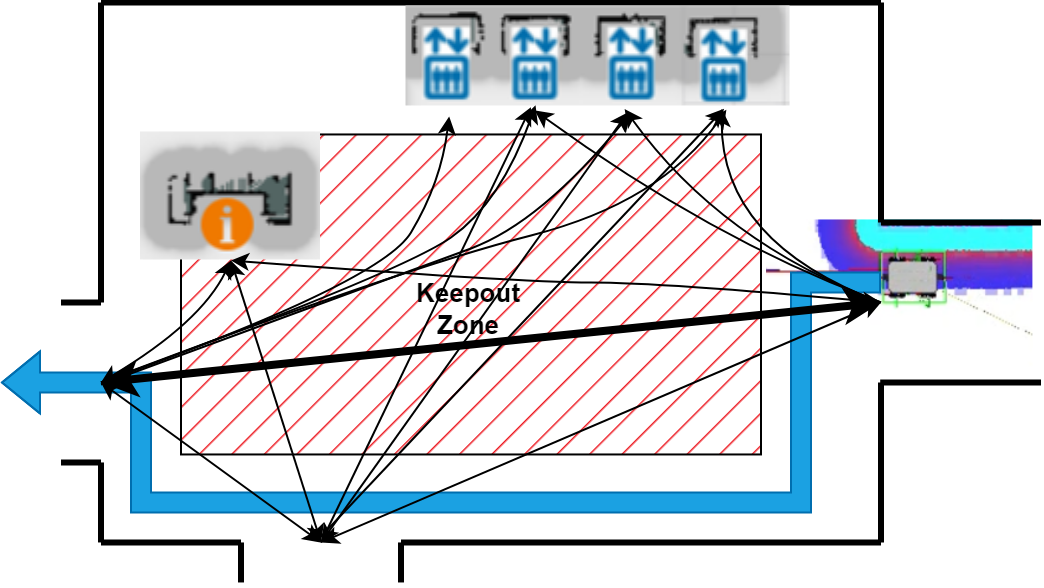
\includegraphics[width=0.75\textwidth]{figures/10_introduction/straight_path_problem.png}
    \caption[The problem of shared human-robot areas]{The problem of shared human-robot areas. Black arrows show the main routes of human traffic. The red keepout zone should be avoided to prevent conflicts. The blue path has fewer conflicts and is more predictable.}
    \label{fig:straight_path_problem}
\end{figure}

Figure \ref{fig:straight_path_problem} shows an example scenario for a robot driving in a public area. This is a typical lobby or waiting room in a hospital. Naturally, nurses and patients take the shortest path between doors or other points of interest such as elevators or an information desk. This results in the paths shown with black arrows. If a robot is introduced into this environment, classical path planning approaches would plan a path that is also the most direct and shortest in terms of path length. In this scenario, this would not be the best option and may even be slower than other alternatives. A direct path would cause many conflicts with main traffic routes, requiring the robot to slow down or even stop and replan its path to avoid collisions with humans. Thus, the goal of this work is to find paths that are predictable and avoid high traffic areas, as well as to provide a metric to measure this effect. Predictability is achieved by performing motions that other humans in the area would expect from a robot, such as moving in a straight line parallel to a wall. Therefore, the blue path in the figure above would be better. The red keepout zone indicates the area the robot should avoid to prevent collisions.

As a conclusion from the presented problem statement, it is clear that multi-floor navigation is a huge benefit for the productivity of service robots and that the need for a predictable path that does not disturb the public space is essential to ensure safety and reduce the risk of collisions and accidents. Therefore, the two main research questions addressed in this thesis are:
\begin{enumerate}
    \item How to navigate in complex multi-floor environments?
    \item How to plan paths that are straight and predictable?
\end{enumerate}

The scope of this work is limited to the development of a planner that plans a priori with previously collected information, as opposed to a controller that follows the planned path and adapts to dynamic obstacles. The main assumption is that a map of the entire environment has been previously recorded and provides a complete representation of the plannable space.

%% ==============================
\section{Use Case PeTRA}
\label{sec:use_case}
%% ==============================
The use case of this work is a mobile robot that will be used to assist staff with patient logistics in care facilities. This includes tasks such as delivering medication and transporting a patient to examinations. This work is part of the \gls{petra} research project funded by the \gls{bmbf} \cite{bmbf-internetredaktion_bekanntmachung_2018} and developed at the \gls{iras} of the \gls{hka}.

Transporting patients from ward to examination is part of the daily routine in a hospital. This manual transport is usually performed by trained nurses who cannot perform nursing activities while they are absent from the ward. To reduce transfer time, patients are moved through the hospital in beds, even though some of them would be able to walk. This transfer method does not promote patient mobility, nor does it allow patients to decide if and how they want to walk. "\Gls{petra} is designed to relieve caregivers of time-consuming and labor-intensive patient transport and give them more time for qualitative care" \cite{petra-konsortium_personen-transfer_2022}. To achieve this goal, an autonomous mobile robot was developed in collaboration with industry partners and three hospitals. \Gls{petra} offers different transfer modes to adapt to each patient's needs, see Figure \ref{fig:multi_mobility_methods}. Autonomous patient transport is realized with sensory coupling for free walking or with the support of a rollator (center) and a modular platform for wheelchairs (left). This platform is used for safe wheelchair transport and can be coupled. In addition, an integrated robotic arm performs service tasks (right). These include transporting medications or blood samples between the storage area and the wards.

\begin{figure}[h]
    \centering
    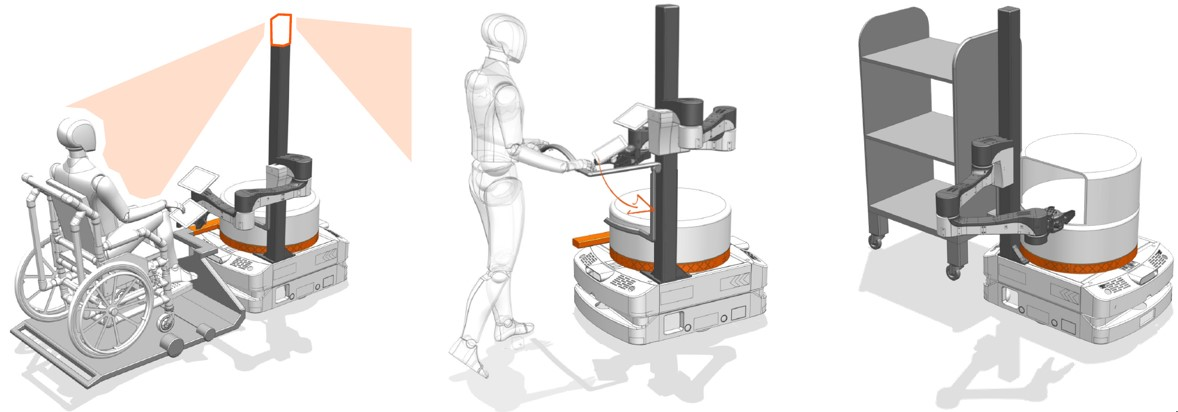
\includegraphics[width=\textwidth]{figures/10_introduction/PeTRA_transport_modes.jpg}
    \caption[Multi-mobility methods of PeTRA]{Multi-mobility methods of PeTRA: wheelchair transport (left), sensory coupling (center) and material transport (right).}
    \label{fig:multi_mobility_methods}
\end{figure}

To demonstrate the feasibility and economic viability of autonomous transportation in hospitals, \gls{petra} must be able to perform tasks between arbitrary locations in this complex environment. This work allows \gls{petra} to navigate across multiple floors while following a predictable path.

%% ==============================
\section{Structure of this Thesis}
\label{sec:structure}
%% ==============================
The following work is structured as follows: Chapter \ref{sec:state_of_the_art} provides an overview of the state of the art in multi-floor path planning for mobile robots. It also discusses the limitations of existing approaches and presents the research gap. Chapter \ref{sec:methods} describes the methods used to evaluate the results of this work. The concept of hierarchical and straight path planners is presented in Chapter \ref{sec:concept}, followed by their implementation in Chapter \ref{sec:implementation}, where the algorithms used are presented. Chapter \ref{sec:results} presents the results of the work and a comparison with related work in the field. Chapter \ref{sec:discussion} discusses the limitations and applications of the results. Finally, Chapter \ref{sec:conclusion} summarizes the contributions of the thesis and gives recommendations for future work.